\begin{figure}[h!]
\centering
\caption{Proyecciones del Balance Primario del GNC}
\label{fig:bp}
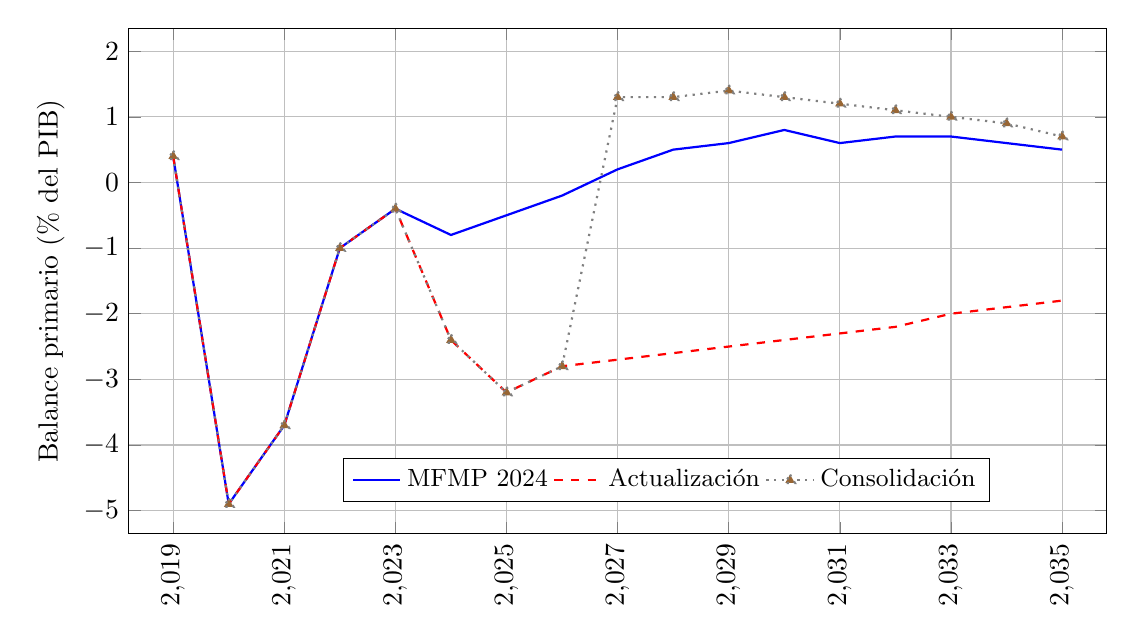
\begin{tikzpicture}
\begin{axis}[
    width=14cm,
    height=8cm,
%    xlabel={Año},
    ylabel={Balance primario (\% del PIB)},
    xmin=2019, xmax=2035,
    ymin=-5, ymax=2,
%    xtick={2019,2020,...,2035},
    xtick={2019,2021,...,2035},
    xticklabel style={rotate=90,anchor=east},
    ytick={-5,-4,-3,-2,-1,0,1,2},
    grid=both,
    legend style={at={(0.55,0.15)},
    legend style={font=\small},
    anchor=north, legend columns=3},
    enlargelimits=0.05,
%    title={Escenarios del balance primario (\% del PIB)}
]

% Datos MFMP
\addplot+[mark=none, color=blue, thick] coordinates {
(2019,0.4) (2020,-4.9) (2021,-3.7) (2022,-1.0) (2023,-0.4)
(2024,-0.8) (2025,-0.5) (2026,-0.2) (2027,0.2) (2028,0.5)
(2029,0.6) (2030,0.8) (2031,0.6) (2032,0.7) (2033,0.7) (2034,0.6) (2035,0.5)
};
\addlegendentry{MFMP 2024}

% Datos Actualización
\addplot+[mark=none, color=red, thick, dashed] coordinates {
(2019,0.4) (2020,-4.9) (2021,-3.7) (2022,-1.0) (2023,-0.4)
(2024,-2.4) (2025,-3.2) (2026,-2.8) (2027,-2.7) (2028,-2.6)
(2029,-2.5) (2030,-2.4) (2031,-2.3) (2032,-2.2) (2033,-2.0) (2034,-1.9) (2035,-1.8)
};
\addlegendentry{Actualización}

% Datos Consolidación
\addplot+[mark=triangle*, color=gray, thick, dotted] coordinates {
(2019,0.4) (2020,-4.9) (2021,-3.7) (2022,-1.0) (2023,-0.4)
(2024,-2.4) (2025,-3.2) (2026,-2.8) (2027,1.3) (2028,1.3)
(2029,1.4) (2030,1.3) (2031,1.2) (2032,1.1) (2033,1.0) (2034,0.9) (2035,0.7)
};
\addlegendentry{Consolidación}
\end{axis}
\end{tikzpicture}
\par\footnotesize{\textit{Fuente: Elaboración propia con base en MFMP 2024, Balance del GNC y Deuda del GNC, Ministerio de Hacienda.}}
\end{figure}
